\documentclass[conference]{IEEEtran}

% Use of outside images
\usepackage{graphicx} 
% Use text inside euqations
\usepackage{amsmath}

\usepackage{balance}
\usepackage{float}
\floatstyle{plaintop}
\restylefloat{table}

% Correct bad hyphenation here
\hyphenation{op-tical net-works semi-conduc-tor}

% Begin the paper here
\begin{document}

% Paper title
% Can use linebreaks \\ within to get better formatting as desired
\title{Automatically Eliciting Requirements From Forums: A Hearthstone Case Study}

% Authors names
\author{\IEEEauthorblockN{Jordan Ell}
\IEEEauthorblockA{University of Victoria,
Victoria, British Columbia, Canada \\ jell@uvic.ca}
}

% Make the title area
\maketitle


\begin{abstract}
Requirements elicitation has been recognized as a crucial activity in any software development project. 
Unfortunately, collecting and examining new requirements can often be a difficult manual task when
information is distributed across numerous stakeholders. As a result, new automated requirements elicitation tools
have started to surface which take advantage of information sharing tools, such as online forums and wiki pages.
In this study, I look to create a new methodology for automatically eliciting requirements from online forums in
order to better support developers and remove the manual process of finding said requirements with human work effort.
I perform a case study of a video game Hearthstone: Heroes of Warcraft in which online forum postings are used to
extract requirements which the users would like to see fulfilled by the game developers. After analyzing 4000 posts 
from the forum, 911 new requirements were found with an accuracy of 13\% validity. These results show the beginnings
of an emerging area of research which requires much future work and elaboration.
\end{abstract}


\section{Introduction}

% Broad
As software projects grow larger and involve more
stakeholders, project managers often look to open discussion forums to elicit requirements
and otherwise communicate with other stakeholders~\cite{Wanner:2011:FEU}.
Large software projects which have hundreds, thousands, or even millions of users
often have large online communities which discuss, debate, and even express joy
for their software product. Often, these communities are looked to for improvements
to the software products through both bug reports and, perhaps more importantly, requirements
through feature requests or tweaks to the software~\cite{Shin}. The larger these communities are, more
often the more valuable they become to the software developer as more and more minds can express
their opinions and wants.

% Specific
For video game development, hearing from the community is extremely important~\cite{Ruggles:2005:OCB}. Almost any
video game creators will employ a ``Community Manager'' in order to monitor their online
communities and communicate the needs and wants of the users to the development teams and
business teams. This job can be a tedious task, as it is up to the community manager to 
go through thousands, if not millions, of online discussions in order to find out what
users really want from the game and how they can go about implementing these 
requirements~\cite{Gottipati:2011:FRA}.
This may involve many hours each day going through post after post to identify requirements
that the community of users has created for the developers.

% Quick overview of related
Some work in the past has looked at automated techniques in the field of requirements and
features with varying levels of success in order to alleviate some
pressure off of these community managers. Noll et al.~\cite{Noll:2010:REO}
analyzed an open source software projects to
identify by whom and where requirements are proposed. Boutkova et al.~\cite{Boutkova}
used some semi-automated
techniques to identify features to be implemented in requirements specifications. Clealand-Huang
et al.~\cite{Cleland-HuangDDC09} also looked at creating a forum management system which can help identify requirements
by a domain expert. All of these approaches have not been fully automated and require some
human intervention for their results to be accurate.

% Question
In order to remedy this manual and slow process with full automation, I ask the research question: 
``Can software requirements be automatically elicited from online forums?''

% Quick results
To address this question, I perform a case study of the video game Hearthstone: Heroes of Warcraft,
which is a created by Blizzard Entertainment. By scraping their online forums, and applying some
natural language processing techniques, I was able to extract 911 new requirements from the forums 
with a validity accuracy of 13\%. 

% Outline
The rest of this paper is outlined as follows. Related work will first be discussed to underline 
how this research is novel. Methodology will then be presented to explain exactly what steps were taken
for the research. Results and discussion will then follow to go over what was found and what steps
can be take in the future to improve these results.


\section{Related Work}

As was stated in the introduction, some research has been put into this area~\cite{Ambriola:1997:PNL}
even though most
has not been towards full automation of the requirements gathering process. Cleland-Huang et al.
have extensively studied how online forums can be used in assistance with the requirements gathering
process. They have been able to use data mining and recommender systems~\cite{2008}, as well as
feature requests from online forums to help community managers communicate the needs of stakeholders
to developers~\cite{Cleland-HuangDDC09}.

Hariri et al.~\cite{HaririCMCM13} have looked into using cross domain products and their feature
listing to recommend requirements to other products in that domains. This allows requirements to
be found through online text by simply comparing what features similar products have. Taylor et
al.~\cite{Taylor} looked into extracting requirements from similar product's product descriptions.
This is again a sort of comparison between products to find new requirements. Both these methods
involve knowing where requirements are unfortunately and do not solve the issue of pure 
open text requirements mining which is found is online forums.

Castro-Herrera et al.~\cite{Castro-Herrera:2009:RSD} have also looked at online forums for
extensive topic analysis as well as a recommendation system for topics based on text. Hindle et
al.~\cite{hindle} have also looked at topic extraction from free text and requirements as to
their meaningfulness to managers and developers. Again both of these research areas show promise
towards automatic elicitation of software requirements.

\section{Methodology}

The basis of this approach is to extract highly favored requirements from an online forum which supports
user needs of a software product. As was said, I have selected the video game ``Hearthstone: heroes of Warcraft'',
hereon known as Hearthstone, as my experimental software application. Hearthstone is produced by a large
video game manufacturer known as Blizzard, who is the produced of many top tier video games and who has an
extensive online community. The reason this game was selected was for two reasons. One, Blizzard has a large
community presence in their online forums for all the game products. This helps me by creating a very
rich and diverse test bed of forum posts from which information can be collected. Second, Hearthstone was
selected because of the phase in which its game development was in. At the time of this research, Hearthstone
had been in open beta for 2 months and was roughly 1 month short of its official launch date. This put my
research in a perfect position where players were still finding bugs, tweaking the game play settings, 
assessing the visuals and so much more. Because of this, my results had the highest chance of finding
exactly what players wanted to change, and with some sense of urgency as the game was about to make its
debut.

\subsection{Information Collection}

% Crawling
Once the game was selected, information had to be collected. I needed to obtains all of the forum posts
for this game and store them in some way which was to be used later. Since Blizzard does not have a public API
for accessing their online forums, or their content, I had to crawl and scrape the information myself. To
do this, I used the python library called BeautifulSoup\footnote{http://www.crummy.com/software/BeautifulSoup/}
 in order to extract the information I needed. I extracted
the following information from every post:

\begin{table}[h]
\begin{center}
\begin{tabular}{| l | p{6cm} |}
\hline
User & The name of the user making the post \\
Body & The content of the post \\
Created & The time which the post was created \\
User Title & The forum title of the user if applicable (moderator, admin, etc) \\
Discussion ID & This ID of the discussion which the post belongs to \\
\hline
\end{tabular}
\end{center}
\caption{Information collected on posts.\label{tab:posts}}
\end{table}

\begin{table}[h]
\begin{center}
\begin{tabular}{| l | p{6cm} |}
\hline
Title & The name of the discussion thread \\
Topic & The forum topic in which the thread was created in \\
Created & The time which the discussion was created \\
\hline
\end{tabular}
\end{center}
\caption{Information collected on discussions.\label{tab:discussions}}
\end{table}

Once the information was extracted, I simply stored it in a PostgreSQL database for future use. It can
be seen in Table~\ref{tab:posts} and Table~\ref{tab:discussions} that information about posts and their
discussion threads was collected. A total of 44,381 posts were scraped from 5495 discussion threads. 

\subsection{Technical Approach}

After the information had been collected, a technical approach for extracting the requirements was created.
First, some aspects of plagiarism techniques~\cite{Leung:2007:NLP} were used in order to group posts into unique topics. To start,
posts were split up into individual sentences to be further analyzed. Analyzing at the sentence level allows
me to have my analysis in line with my results, which are requirements sentences (this will be seen later) The
downside of analyzing on a per sentence basis is the loss of context as to what the user was writing about
may occur. Once sentences were obtained, a plagiarism technique of finding similar nouns in sentences was
used to identify similar sentences. For this, each noun from each sentence was extracted into that sentence's
bag of nouns. From here, the cosine similarity formula was used to identify which bag of nouns were similar. 
A threshold of 60\% similarity was used as the cut off, meaning that sentences had to be at least 60\% similar
in their nouns in order to be grouped together.

\begin{equation}
\text{Similarity} = \frac{ A \cdot B }{||A|| x ||B||}
\end{equation}

As a side note, in order to pick out the nouns of each sentence, the python library NLTK\footnote{http://www.nltk.org/}
was used extensively.
This is a natural language processing toolkit for python which has a large suite of tools. For this methodology,
the notion of ``chunking''~\cite{Collobert:2011:NLP} was used. Chunking is essentially breaking a sentence apart and identifying which English
lexicographical identifier can be applied to each word of the sentence. This allows me to identify the nouns.

After the sentence have been divided into their groups of similarity, it is time to identify the requirements,
of each group. For this, I again used the NLTK library and used a methodology known as 
``phrasing''~\cite{Collobert:2011:NLP}. Phrasing
essential groups parts of sentences together into their applicable phrase type.

\begin{figure*}[tb!]
\centering
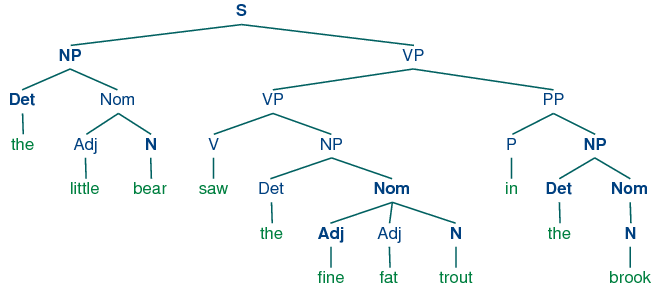
\includegraphics[width=0.9\textwidth]{images/phrase}
\caption{An example of phrasing. We can see clearly a noun and a verb phrase.\label{fig:phrase}}
\end{figure*}

As can be seen in Figure~\ref{fig:phrase}, in order to complete phrasing, chunking is simply applied
follow by a grammar of the English language. We can see that a verb phrase has been constructed as well
as a noun phrase. This will end up being the sentence structure needed for or final step of requirements
extraction. Since requirements often has a structure of ``Some object should perform some action'', identifying
the noun and verb phrases of our sentences is now key. For now, we simply trim each group of similar sentences
to those which have this type of sentence structure.

Now obviously at this point, we run into an issue of trimming real requirements which just do not fit out structure.
This is a real problem an will be addresses in the future work section. We also now see the issue that while sentences
have a noun and verb phrase, the extraction of these phrases can be quite difficult. Since English has
a larger amount of flexibility, not all sentence structures can be identified using this method, as a grammar must
be provided which fits this structure. Again this limitation will be addressed later in this paper.

Now that sentences with the correct requirement structure have been found, simple key word analysis is used 
to complete this approach. As it can be seen in Figure~\ref{fig:phrase}, a verb phrase begins with a verb. 
We can use this knowledge to identify request type sentences. I created a list of words:

\begin{itemize}
  \item Should
  \item Add
  \item Could
  \item Allow
\end{itemize}

which can be used to identify sentences which have a request like nature. This allows me to find sentences
which as asking for some action to be performed (verb phrase) on some object (noun phrase). At this
stage in the research, the first sentence found in the similar group of sentences to have one of the aforementioned
keywords as its verb phrase verb is chosen as the requirement to represent this bag of sentences. We have
now automatically elicited requirements from online forum data.

\subsection{Validation}

In order to validate what was found to be a requirement automatically, a simple inter-rater reliability~\cite{gwet2001handbook}
validation was applied
with three judges (myself and two external judges). All three judges had domain knowledge of Hearthstone as all three
had played the game before and therefor would be able to interpret the requirements correctly. 100 requirements were selected randomly 
to be tested. These random 100 only had one constraint, and that was that they come from sentence groups
which has a minimum of 100 similar sentences. Each judge was given the list of 100 requirements and asked to give a binary result of Yes or No. A Yes
indicated that the judge found that the requirement was a real requirement for Hearthstone and that they could easily
understand it. A No indicated that the judge either could not understand the requirement or that it was not a requirement
at all.

\section{Results}

From the Hearthstone online forums, a total of 44,381 posts were scraped from 5495 discussion threads. Of
these posts, 4000 were analyzed for the interim results of this paper. (The total posts elicitation is still
running at the time of writing this paper.) From these 4000 posts, 911 requirements were found. A threshold of
100 sentences in the similarity group was used as a cut off to only use those requirements which are from
tis post popular discussions on the forum.

To give a clear picture of the results, I have selected the following as a representative sample space of the
types of requirements found:

\begin{enumerate}
  \item The 0/1 Taunt is more annoying and so therefore should have a lower mana cost
  \item Arena should reward versatility and making the best with the least
  \item They should ban or restrict the card like in MTG but never nerf
  \item So I think low-balling the cost, it should cost at least 8
  \item Needless to say, either the mana cost of these cards needs to increased or the priest should only be allowed to run one of each
  \item Turn 10 is when big plays should happen
\end{enumerate}

As it can be seen, requirements found range in usefulness. The first two above represent the cream of the crop found
by this automatic technique. To those with domain knowledge, they are clear and resemble an easy to understand
requirement structure often found in formal documentation (Some object should perform some action). The third requirement,
shows how meta requirements can be found. The fourth requirement shows a large downfall of this methodology, that being
the word ``it'' is often used and refers to an object of a different sentence which ultimately renders this requirement,
on its own, useless. The same can be seen for requirement 5. And finally, requirement 6 shows that even with a matching
sentence structure, a sentence may itself not be a requirement.

As per the validation of the requirements found, the inter-rater reliability methodology was used as previously stated.
From the 100 requirements manually analyzed, an intersection of agreement between all three judges was found to be 13\%
for real requirements. This means that the methodology presented in this paper can be seen to have an accuracy of 13\%.
As additional 3\% of requirements were seen to be accurate from only two of three judges and an additional 5\% were seen
to be accurate be a single judge.

\section{Discussion and Future Work}

While the methodology presented in this paper can be considered a good start in automatic requirements elicitation, 
many limitations exist as can be seen in the final 13\% accuracy rate. Early on in the methodology, we see a large
weakness come along with the phrasing section of work. Here, I require that a sentence take the structure of noun
phrase followed by a verb phrase. First off, in order to extract this structure, a grammar must be used which is compliant with
the sentence structure. This means that a grammar must be created and be available for every type of sentence that
can be constructed using the English language. This is quite a lofty task. For this research paper, I simply used those
(limited) grammars that came ``in the box'' with NLTK. This has a large consequence of missing potential sentences
which do not fit this grammar. This inevitably leads to missing requirements down the road. To fix this issue, a large
catalog of English sentence grammars must be created in order to properly parse all English sentences by chunking and
phrasing. This may be an extremely large (if not impossible~\cite{shieber1985eac}) task which would require 
manual intervention but may benefit not only requirements
elicitation, but all of natural language processing.

A second consequence of this methodology is the large number of false positives that can be seen in the final results.
Sure a human with domain knowledge of the software product can easily see which requirements are valid and which are not,
but the ultimate goal should be a low number of false positives so that the original problem of humans looking for requirements
manually could be eliminated. As it was seen in the sample of results, many sentences which fit the structure outlined in
the methodology are actually not requirements. The result ``Turn 10 is when big plays should happen'' is obviously not
a requirement, while many other results have the word ``it'' in them, referring to a previous sentence's object but become
unreadable given the sentence oriented results.

In order to fix the issue of the word ``it'' being used so frequently, a pre-processing substitution phase may be a correct 
choice. Here, a find and replace algorithm might be of some use. Finding the word it and then looking back at the current and
previous sentences to find the  object being refereed to, and then replacing ``it'' with that word. This paper was not able
to try such a methodology because of time constraints but this should be labeled as a key area of future work.

As per sentences which fit correct requirement structure but are not requirements themselves, there may be no way around this
in future implementations. The reason being, is that eventually, requirements must conform to some sort of structure that
can be extracted from plain text. This structure obviously opens itself up to false positives. A potential workaround
would be machine learning with human classification of sentences which are requirements and which are not. This method would
require lots of human intervention and of course would be different across software domains, which may render it useless
as the goal was to eliminate the need for human work.


\section{Conclusion}

Extracting requirements for software from a online community can be a slow and painful process performed manually
~\cite{Gottipati:2011:FRA}.
This paper has presented a method for automatically extracting requirements from an online forum for a video game
called Hearthstone. From the presented methodology, a accuracy of 13\% was found in the requirements that were
automatically elicited. While this can be seen as a promising start, many improvements would need to occur before
this methodology could be used in a large setting.

In future work, pre-processing steps to clean up sentences and give more details about their intent would be needed,
as well as a full catalog of English grammars in order to construct all possible noun and verb phrases.

This paper represents a good first step in processing unstructured text from a community of contributers in order
to automatically elicit requirements from the users community.

\bibliographystyle{}
\bibliography{paper}


% End of the paper
\end{document}